\hypertarget{_benchmark_program_design_BenchmarkProgramDesignGUIFramework}{}\section{G\+U\+I Framework}\label{_benchmark_program_design_BenchmarkProgramDesignGUIFramework}
To benchmark the framework, I will use S\+F\+M\+L to create a graphics application. When running the application, each frame runs many objects. The maximum, minimun, and average F\+P\+S(\+Frame per Second) is what I need for the benchmark. The application allows using different number of threads to run it.\hypertarget{_benchmark_program_design_BenchmarkProgramDesignGUIConfiguration}{}\section{G\+U\+I Configuration}\label{_benchmark_program_design_BenchmarkProgramDesignGUIConfiguration}
When you start the application, it will show you a configuration form like this\+: 
\begin{DoxyImageNoCaption}
  \mbox{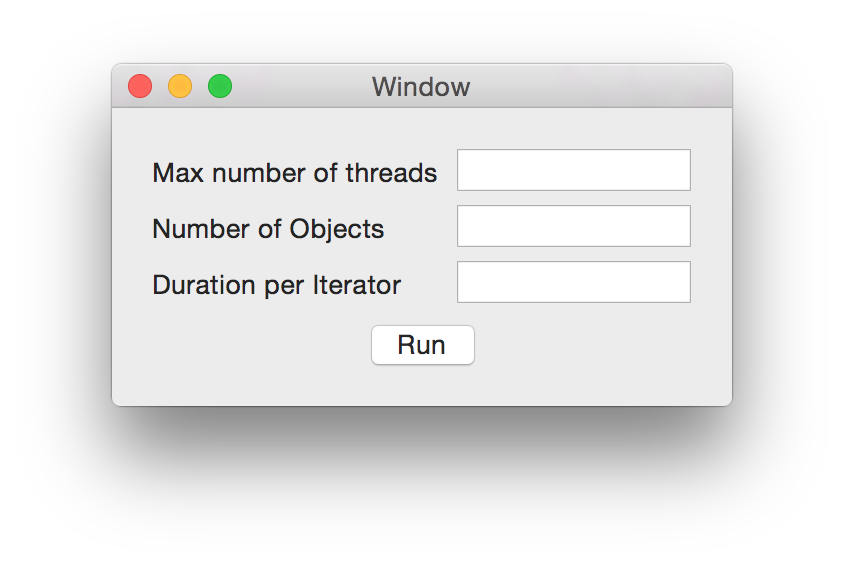
\includegraphics[width=\textwidth,height=\textheight/2,keepaspectratio=true]{DesignBenchmarkProgramDesignGUIConfiguration.png}}
\end{DoxyImageNoCaption}
 The application will run by using one thread to the max number of threads that user configured. The maximun, minimun, and average F\+P\+S will be recorded each iterator. Number of objects and duration for each iterator can be configured by this form.\hypertarget{_benchmark_program_design_BenchmarkProgramDesignOutputs}{}\section{Outputs}\label{_benchmark_program_design_BenchmarkProgramDesignOutputs}
The output is a bar graph which shows all information of the benchmark.
\begin{DoxyItemize}
\item x axis representing number of threads
\item y axis representing frames per second(\+F\+P\+S)
\item values with the maximum, the minimum, and the average.
\end{DoxyItemize}


\begin{DoxyImageNoCaption}
  \mbox{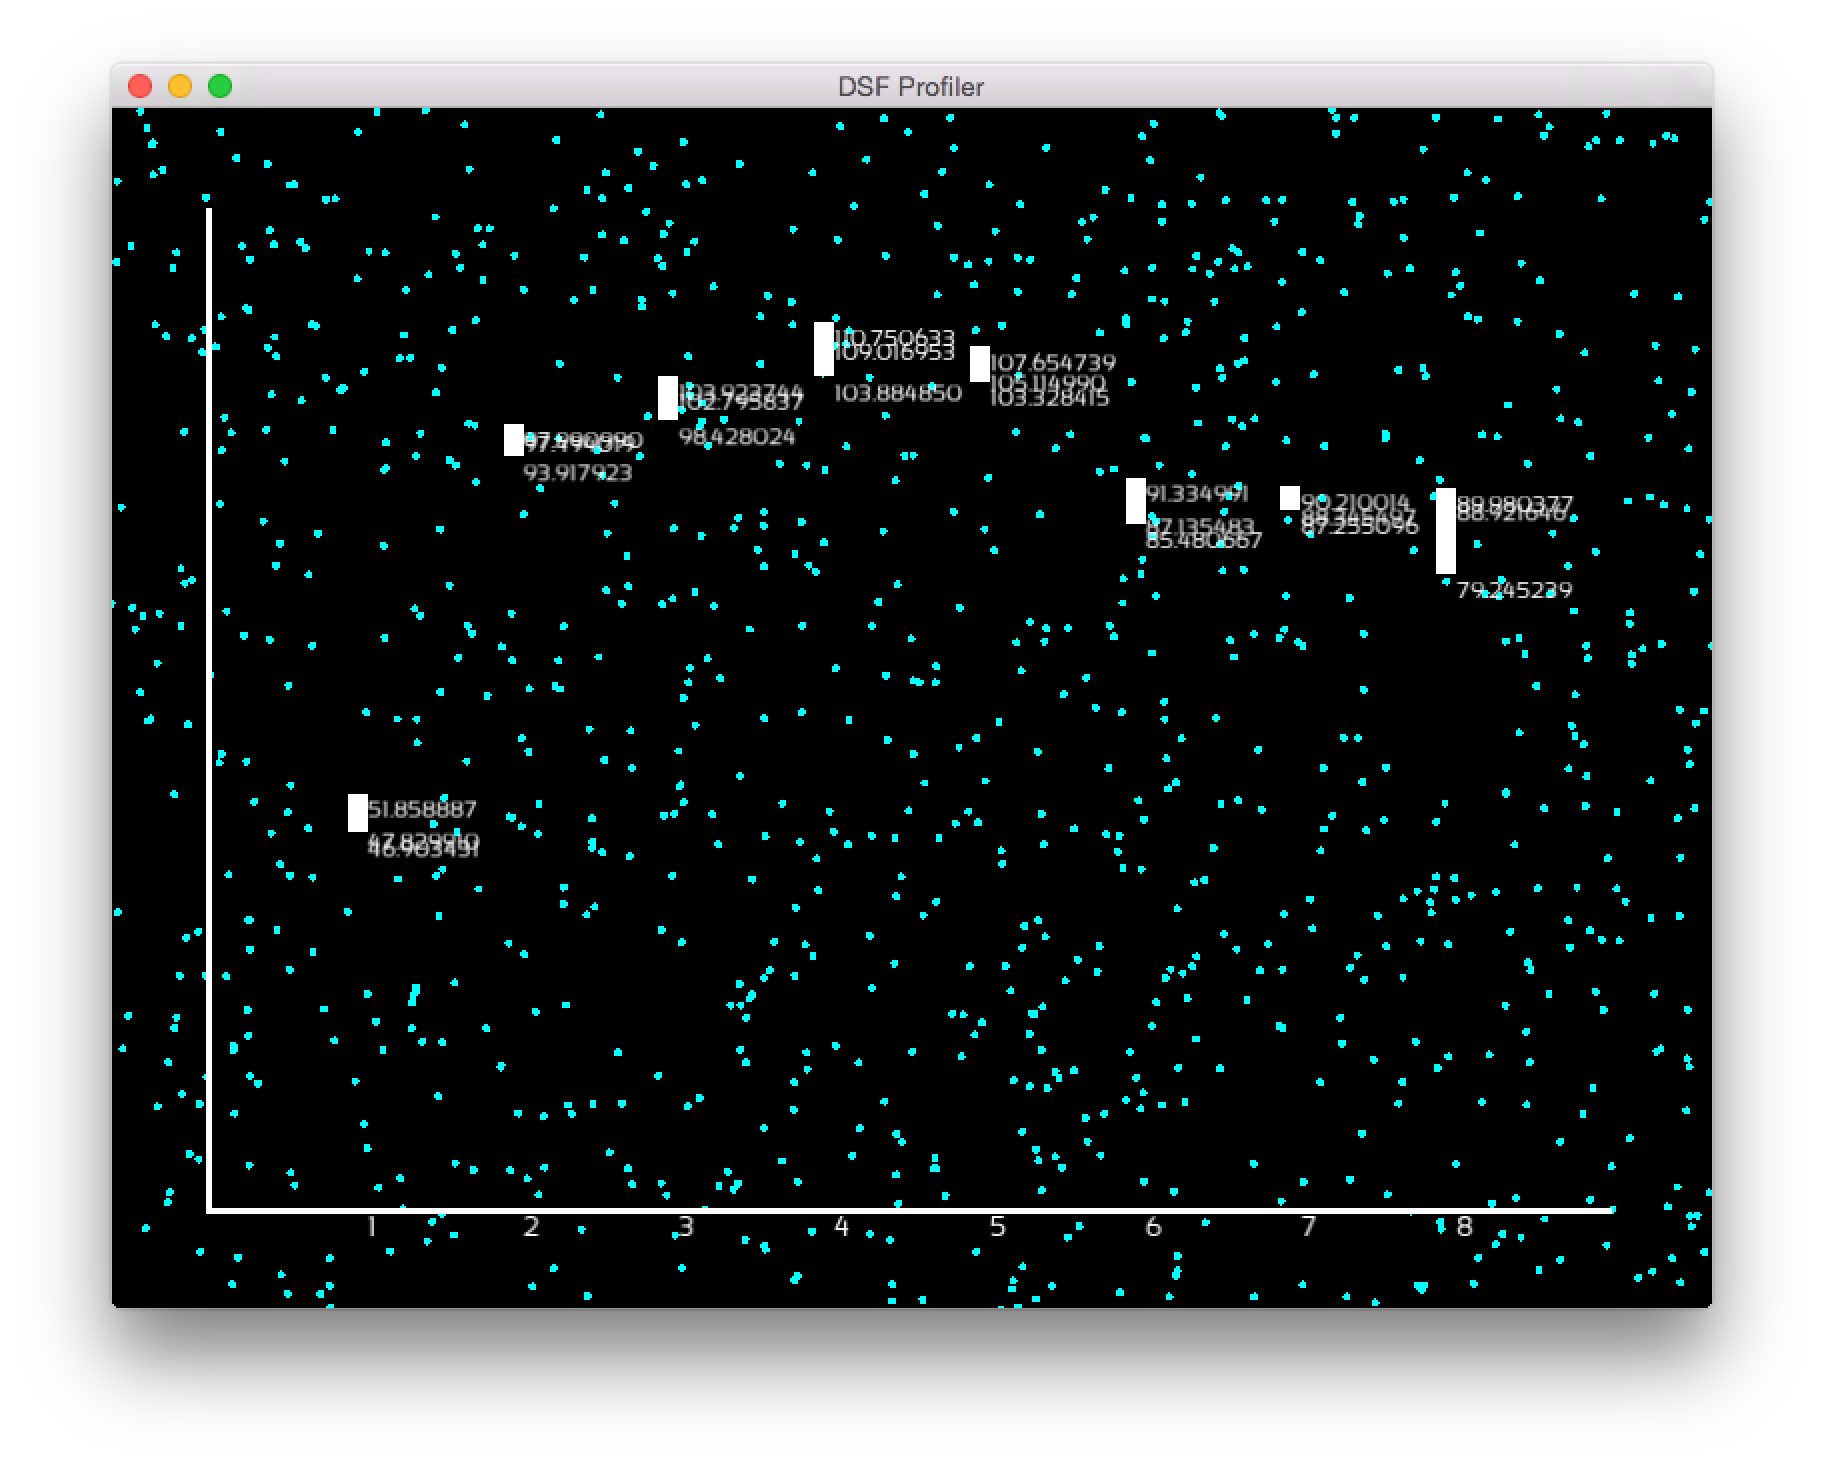
\includegraphics[width=\textwidth,height=\textheight/2,keepaspectratio=true]{DesignBenchmarkOutputs.png}}
\end{DoxyImageNoCaption}
 